\documentclass[hyperref={pdfpagelabels=false}]{beamer}
\usetheme[block=fill]{metropolis}

\usepackage[portuguese]{babel}
\usepackage[utf8]{inputenc} % To use characters such as é without typing é
\usepackage{ctable}
\usepackage{listings}
\lstset{%
  language=Matlab,
  showstringspaces=false,
  basicstyle=\linespread{0.9}\ttfamily,
  keywordstyle=\textbf,
  commentstyle=\color{gray},
  stringstyle=\color{orange},
  numbers=left,
  numberstyle=\tiny\color{gray},
  stepnumber=1,
  numbersep=10pt,
  columns=fullflexible,
  tabsize=3,
  frame=single,
  frameround=tttt
}
\let\Tiny=\tiny % eliminates compilation errors
\usepackage{fontspec}

\title{Laboratório de Matemática Computacional II}
\subtitle{Aula 4}
\author[M. Weber Mendonça]{Melissa Weber Mendonça\\
Universidade Federal de Santa Catarina}
\date{2011}

\begin{document}
\setmonofont{Inconsolata}

\begin{frame}
  \titlepage
\end{frame}

\begin{frame}{Na aula passada...}
   \begin{itemize}
      \item {\texttt{A\textbackslash b}}
      \item {\texttt{inv(A)*b}}
      \item {\texttt{plot(x,y)}}
   \end{itemize}
\end{frame}

\begin{frame}{Exemplos de gráficos}
   Fazer o gráfico das seguintes funções:
   \vfill
   \begin{itemize}
      \item $f(x) = x^4$
      \item $f(x) = \cos{(-3x)}$
      \item $f(x) = e^{-x^2}$
      \item $f(x) = \dfrac{1}{x}$
      \item $f(x) = \dfrac{x^2-3}{x-2}$
      \item $f(x) = \sin{\left(\dfrac{1}{x}\right)}$
   \end{itemize}
   \begin{center}
     \href{listings/graficos.m}{\underline{\texttt{graficos.m}}}
   \end{center}
\end{frame}

\begin{frame}{Título e legendas: {\texttt{title}} e {\texttt{label}}}
  \begin{itemize}
  \item[{\texttt{>>}}] {\texttt{title('y = f(x)')}}
  \item[{\texttt{>>}}] {\texttt{xlabel('x')}}
  \item[{\texttt{>>}}] {\texttt{ylabel('y')}}
  \end{itemize}
\end{frame}

\begin{frame}{Eixos - {\texttt{axis}}}
  Às vezes, precisamos fixar ou modificar os eixos contra os quais fazemos os gráficos. Para isso, podemos usar
  \vfill
  \begin{itemize}
  \item[{\texttt{>>}}] {\texttt{axis}}
  \item[{\texttt{>>}}] {\texttt{axis([x0 x1 y0 y1])}}
  \item[{\texttt{>>}}] {\texttt{axis('auto')}}
  \item[{\texttt{>>}}] {\texttt{axis('equal')}}
  \item[{\texttt{>>}}] {\texttt{axis('tight')}}
  \end{itemize}
  \vfill
  
  Exemplos: $f(x) = \sin{(x)}$
\end{frame}

\begin{frame}{Marcadores}
  \begin{columns}
    \column{4cm}{
      \begin{itemize}
      \item[{\texttt{>>}}] {\texttt{axis('ticoff')}}
      \item[{\texttt{>>}}] {\texttt{axis('ticx')}}
      \item[{\texttt{>>}}] {\texttt{axis('ticy')}}
      \item[{\texttt{>>}}] {\texttt{axis('ticxy')}}
      \end{itemize}
      
      \vskip1cm
      
      Exemplo: $f(x) = e^x$}
    \column{7cm}{
      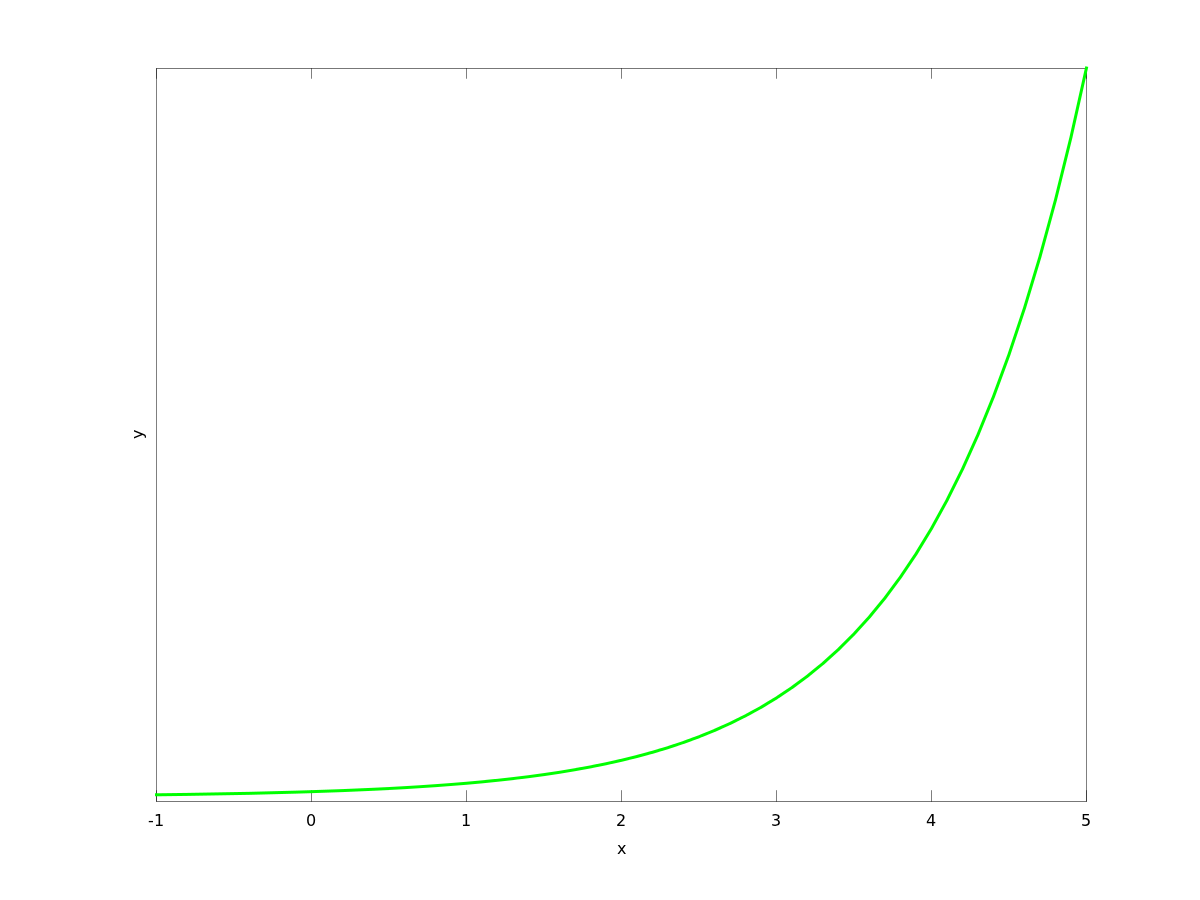
\includegraphics[width=7cm]{img/expx.png}
    }
  \end{columns}
\end{frame}

\begin{frame}{{\texttt{grid}}}
  \begin{columns}
    \column{4cm}{
      \begin{itemize}
      \item[{\texttt{>>}}] {\texttt{grid('on')}}
      \item[{\texttt{>>}}] {\texttt{grid('off')}}
      \item[{\texttt{>>}}] {\texttt{grid('minor')}}
      \end{itemize}
      \vskip1cm
      
      Exemplo: $f(x) = e^x$\\
      Exemplo: $f(C) = \frac{9}{5}C+32$\\}
    \column{7cm}{
      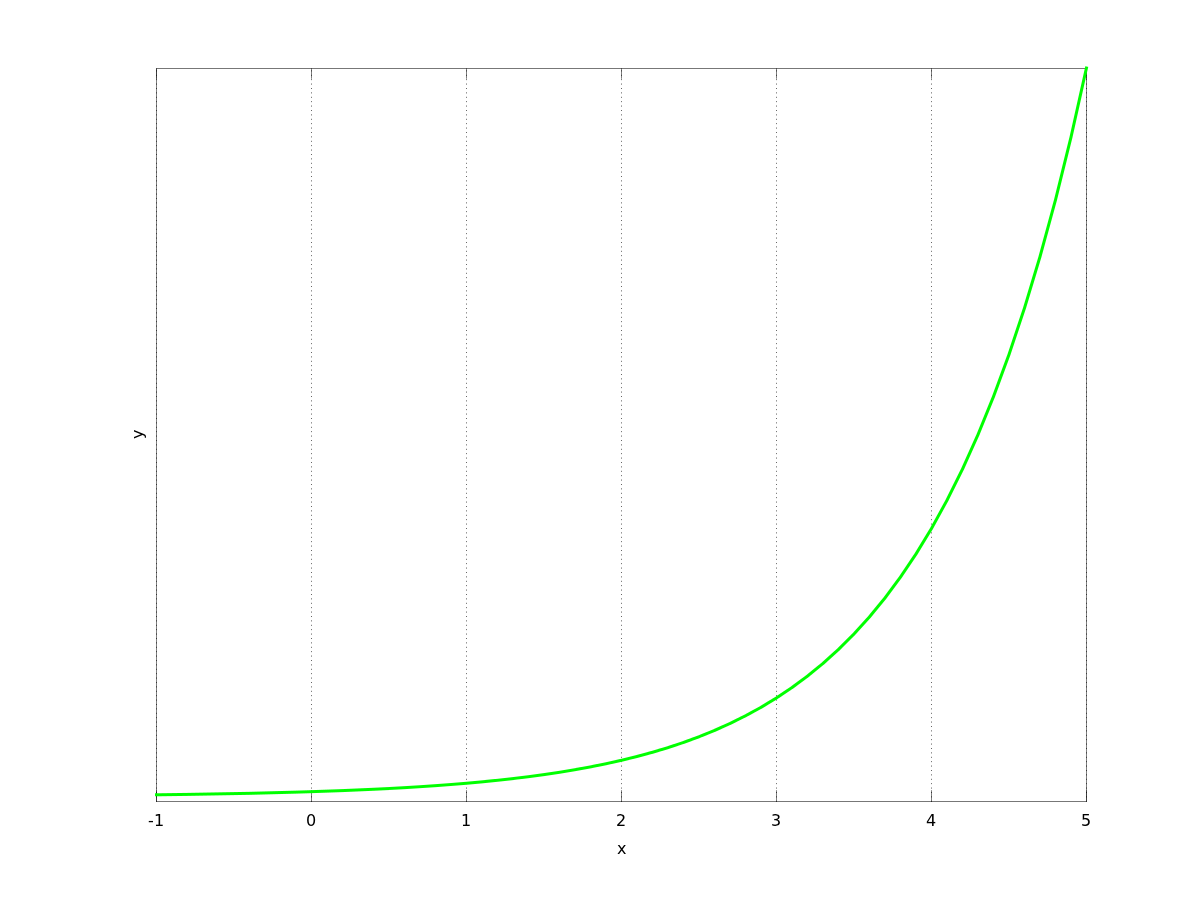
\includegraphics[width=7cm]{img/expxgrid.png}
    }
  \end{columns}
\end{frame}

\begin{frame}{Exercício}
  Fazer os seguintes gráficos:
  \begin{center}
    \only<1>{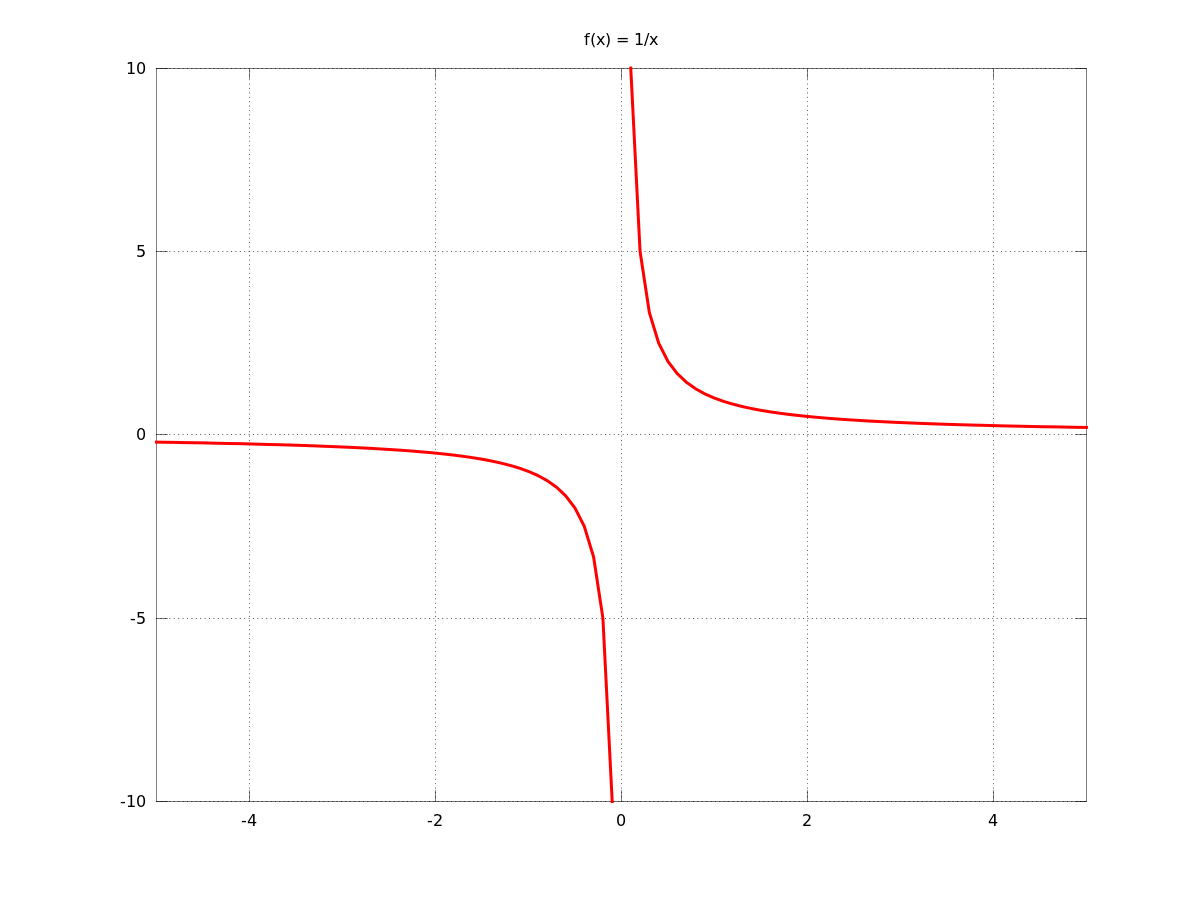
\includegraphics[width=8cm]{img/1overx.png}}
    \only<2>{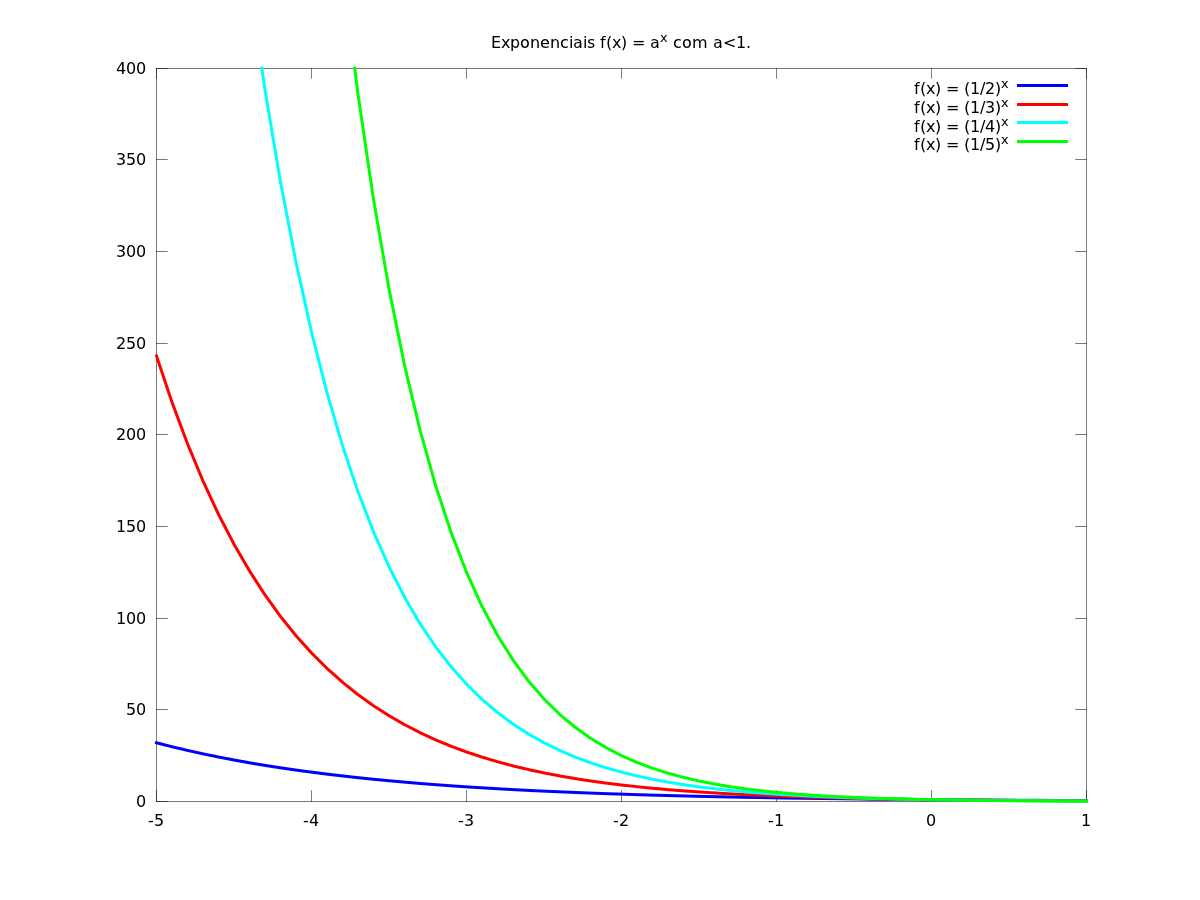
\includegraphics[width=8cm]{img/exponentials.png}}
  \end{center}
  \vfill
  \begin{center}
    \only<1>{\href{listings/umsobrex.m}{\underline{\texttt{umsobrex.m}}}}
    \only<2>{\href{listings/exponenciais.m}{\underline{\texttt{exponenciais.m}}}}
  \end{center}
\end{frame}

\begin{frame}{Ferramentas}
  \begin{itemize}
  \item[{\texttt{>>}}] {\texttt{print('nome.png')}}
  \item[{\texttt{>>}}] {\texttt{legend('legenda')}}
  \item[{\texttt{>>}}] {\texttt{close all}}
  \end{itemize}
\end{frame}

\begin{frame}{Retas: {\texttt{line}}}
  \begin{itemize}
  \item[{\texttt{>>}}] {\texttt{line([1 0],[0 0])}}
  \item[{\texttt{>>}}] {\texttt{line([0 0],[0 1])}}
  \item[{\texttt{>>}}] {\texttt{line([x0 x1],[y0 y1])}}
  \end{itemize}
  
  Exemplo: fazer o gráfico de $f(x) = \frac{1}{x}$ com os eixos $x$ e $y$ desenhados.
  \begin{center}
    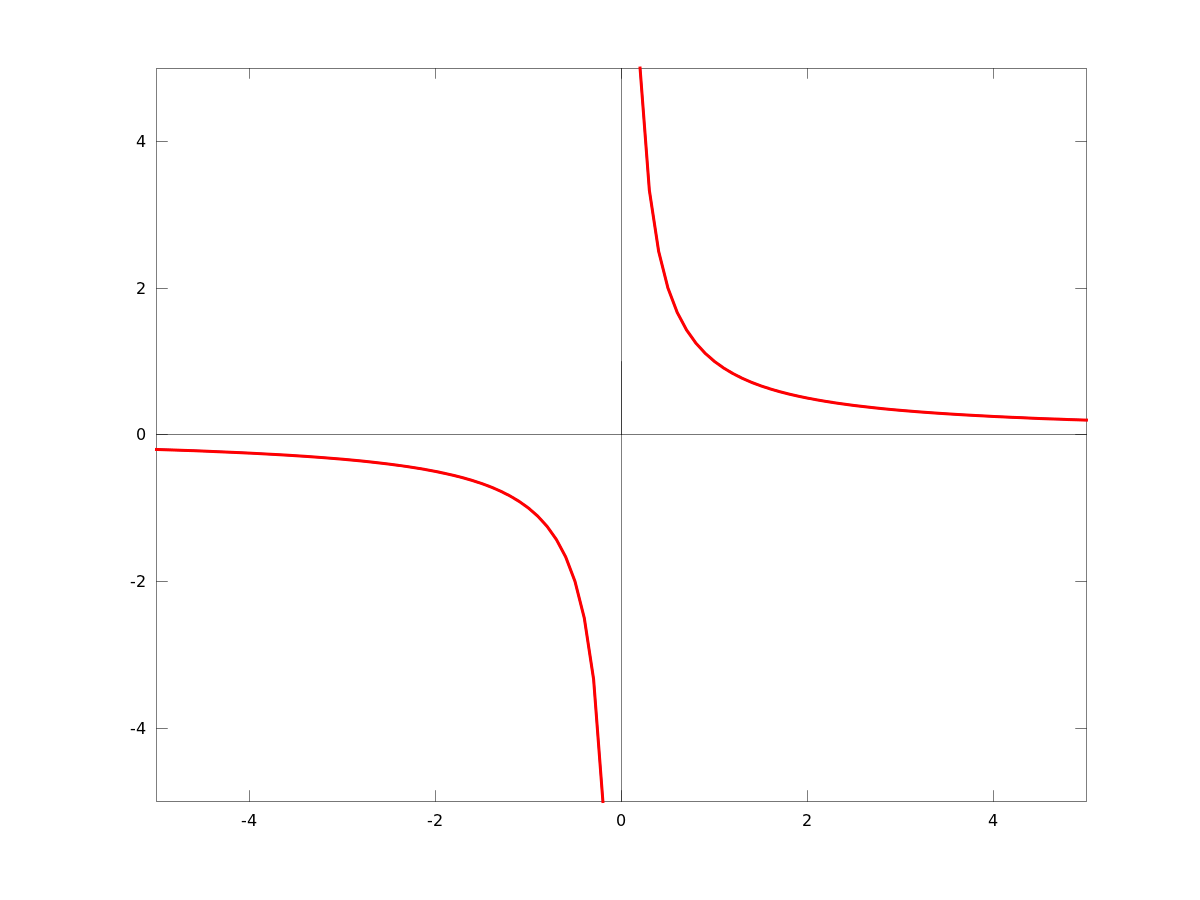
\includegraphics[width=5cm]{img/1overxaxes.png}
    \vfill
    \href{listings/umsobrexcomeixos.m}{\underline{\texttt{umsobrexcomeixos.m}}}
  \end{center}
\end{frame}

\begin{frame}{Exercícios}
  \begin{columns}
    \column{4cm}{
      \only<1>{Faça o gráfico do círculo $x^2+y^2=4$\\\vfill \begin{center}{\href{listings/circulo.m}{\underline{\texttt{circulo.m}}}}\end{center}}
      \only<2>{Faça o gráfico ao lado:\\\vfill \begin{center}\href{listings/triangulo.m}{\underline{\texttt{triangulo.m}}}\end{center}}
    }
    \column{7cm}{
      \only<1>{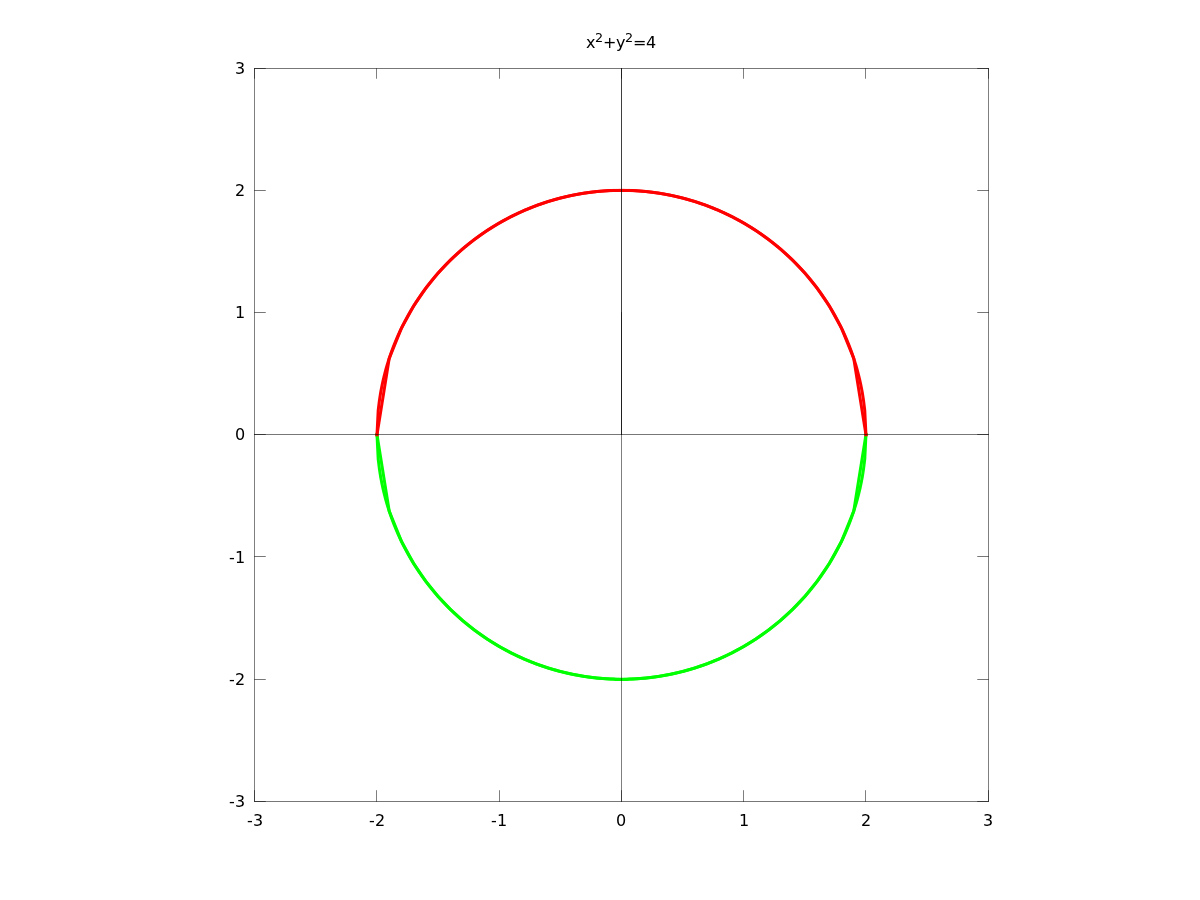
\includegraphics[width=7cm]{img/circulo.png}}
      \only<2>{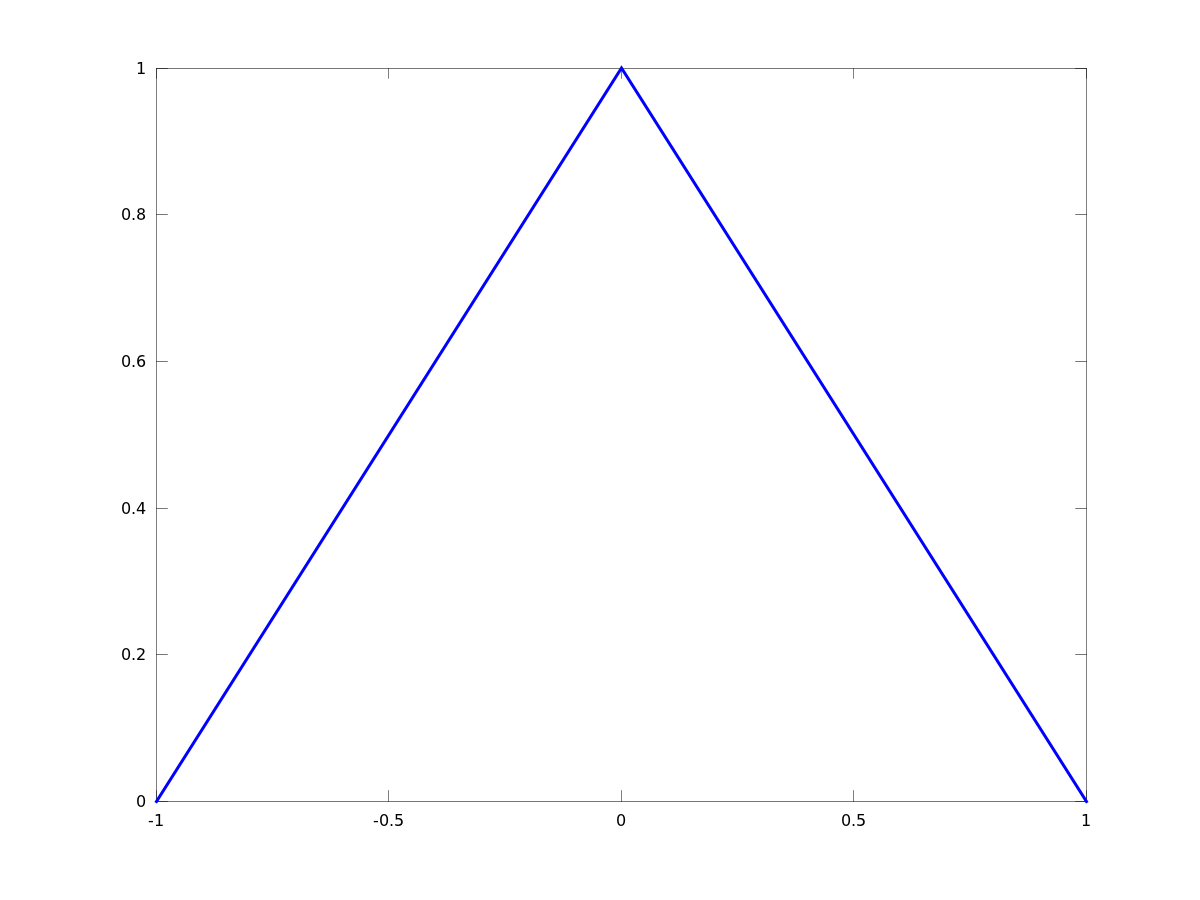
\includegraphics[width=7cm]{img/triangulo.png}}
    }
  \end{columns}
\end{frame}

\begin{frame}{Subgráficos: {\texttt{subplot}}}
  \begin{itemize}
  \item[{\texttt{>>}}] {\texttt{subplot(2,1,1), plot(x1,y1)}}
  \item[{\texttt{>>}}] {\texttt{subplot(2,1,2), plot(x2,y2)}}
  \end{itemize}
  Os gráficos ficam nesta posição:\\
  \begin{center}
    \begin{tabular}{c c c c}
      1 & 2 & 3 & 4\\
      5 & 6 & 7 & 8
    \end{tabular}
  \end{center}
  
  Exemplo: Fazer em uma mesma janela os gráficos das funções seno, cosseno, tangente e cotangente, incluindo os eixos coordenados, títulos para cada gráfico e cores diferentes para cada função trigonométrica. (Dica: pode-se escrever tudo isso em um script!)
  \vfill
  \begin{center} \href{listings/graficostrigonometricas.m}{\underline{\texttt{graficostrigonometricas.m}}} \end{center}
\end{frame}

\begin{frame}{Exercício}
  Fazer uma janela de gráficos contendo os 6 primeiros monômios, sem marcadores de eixo, mas com os eixos coordenados desenhados, contendo títulos para cada gráfico e cores diferentes para cada função.
  \vfill
  \begin{center} \href{listings/graficosmonomios.m}{\underline{\texttt{graficosmonomios.m}}} \end{center}
\end{frame}

\begin{frame}{\texttt{fill}}
  \begin{itemize}
  \item[{\texttt{>>}}] {\texttt{fill(x,y,'x')}}
  \end{itemize}
  \vfill
  
  Exemplo: repetir os seguintes gráficos:
  \only<3>{\begin{center}
\includegraphics[width=3.5cm,height=5cm]{img/smiley.png}\\\vfill \href{listings/smiley.m}{\underline{\texttt{smiley.m}}}\end{center}}
  \only<1>{\begin{center}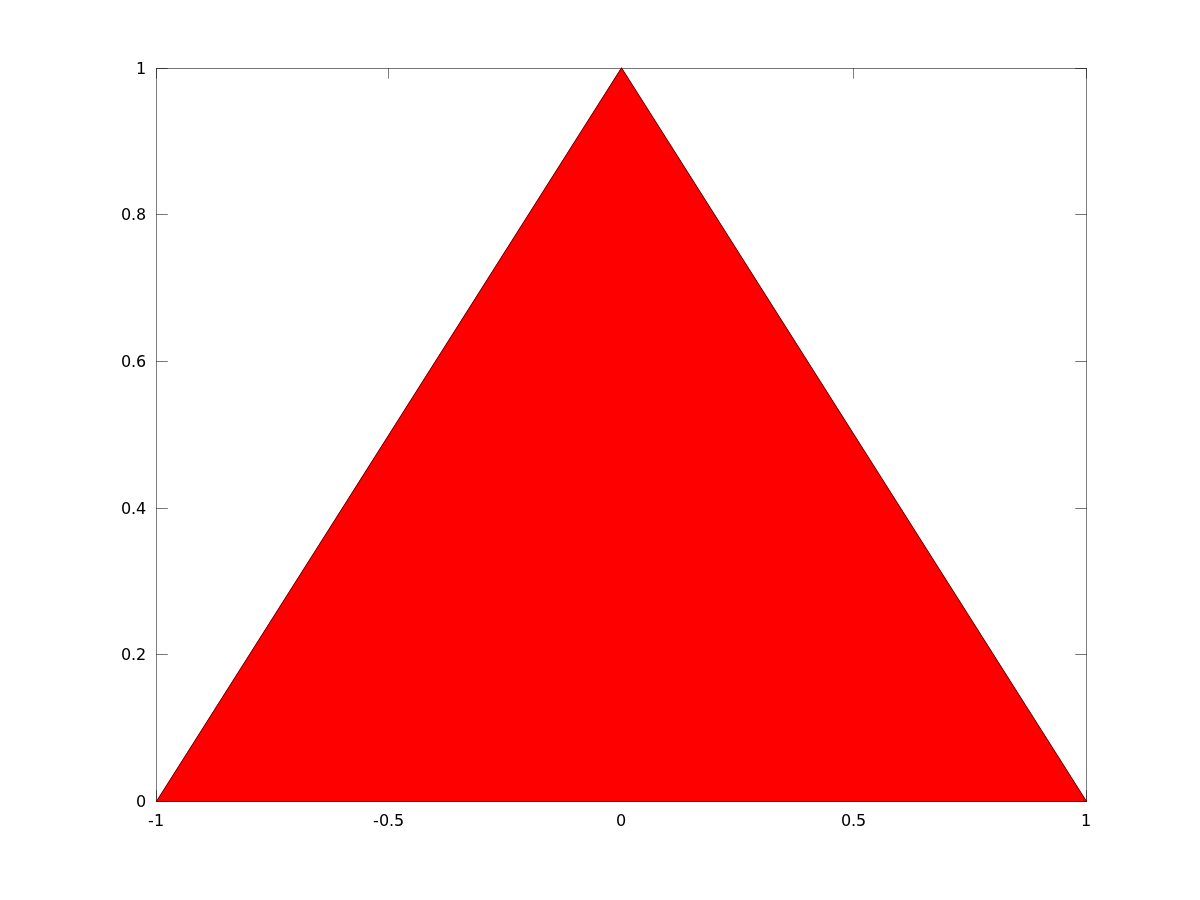
\includegraphics[width=6cm]{img/triangulo_preenchido.png}\\\vfill \href{listings/triangulopreenchido.m}{\underline{\texttt{triangulopreenchido.m}}}\end{center}}
  \only<2>{\begin{center}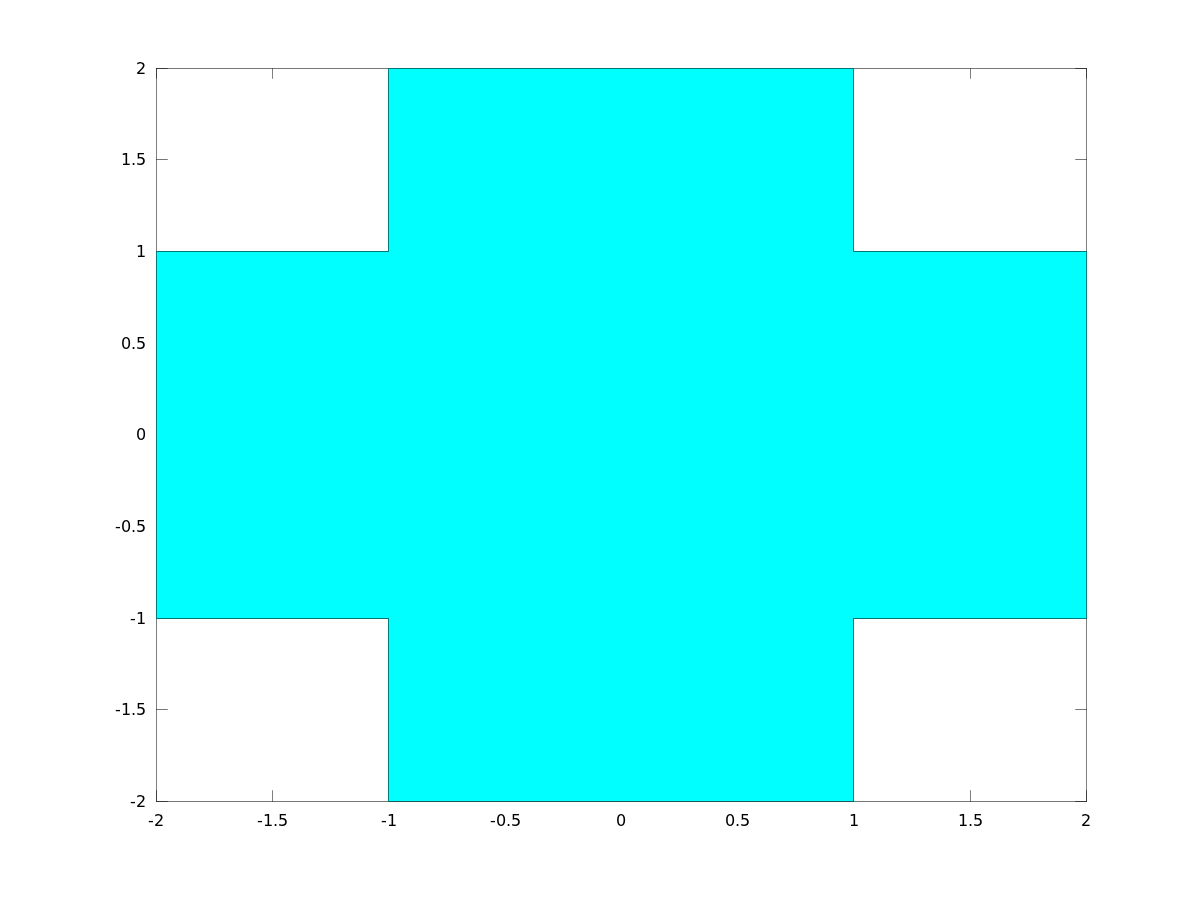
\includegraphics[width=6cm]{img/quadrados.png}\\\vfill \href{listings/quadrados.m}{\underline{\texttt{quadrados.m}}}\end{center}}
\end{frame}

\end{document}
